%=========================================================
% Peripheral : UART
%=========================================================
\section{Peripheral : UART}

\begin{description}

    \item[Overview]\mbox{}\\
        UART is a simple asynchronous Tx/Rx device with a configurable baud rate generator and a 4-depths FIFO buffer for each Tx and Rx. The core logic of the UART is based on SASC (Simple Asynchronous Serial Controller) published on OpenCores (https://opencores.org/projects/sasc) by Usselmann Rudolf. Please see the IP’s document for details. The UART can generate an interrupt request when the Tx FIFO buffer has room to write (not full) or the Rx buffer has at least one data to read (not empty).

    \item[Input / Output Signals]\mbox{}\\
        Input / Output signals of UART are shown in Table \ref{tb:IOSIGNALS_UART}.

%-------------------------------
\begin{table}[H]
    \begin{adjustbox}{scale={0.65}{0.8}}
    \textsf{
    \begin{tabular}{|L{4cm}{2cm}{t}|L{4cm}{2cm}{t}|L{2cm}{1cm}{t}|L{7cm}{6cm}{t}|L{10cm}{6cm}{t}|L{3cm}{2cm}{t}|}
        \hline
        %-------------------------------------
        \rowcolor{LightPurple}
        \textbf{Group} &
        \textbf{Direction} &
        \textbf{Width} &
        \textbf{Name} &
        \textbf{Description} &
        \textbf{Note}
        \nextRow \hline
        %-------------------------------------
        System & input  & ~ & RES & Reset & ~
        \nextRow \hline
        %-------------------------------------
        System & input  & ~ & CLK & System Clock & ~
        \nextRow \hline
        %-------------------------------------
        AHB    & input  & ~                   & S\_HSEL      & AHB Lite Slave Select & ignored
        \nextRow \hline
        %-------------------------------------
        AHB    & input  & \lbrack  1:0\rbrack & S\_HTRANS    & AHB Lite Slave Transfer Type & ~
        \nextRow \hline
        %-------------------------------------
        AHB    & input  & ~                   & S\_HWRITE    & AHB Lite Slave Write & ~
        \nextRow \hline
        %-------------------------------------
        AHB    & input  &                     & S\_HMASTLOCK & AHB Lite Slave Locked Transfer & ignored
        \nextRow \hline
        %-------------------------------------
        AHB    & input  & \lbrack  2:0\rbrack & S\_HSIZE     & AHB Lite Slave Access Size & ~
        \nextRow \hline
        %-------------------------------------
        AHB    & input  & \lbrack  2:0\rbrack & S\_HBURST    & AHB Lite Slave Burst Access & ignored
        \nextRow \hline
        %-------------------------------------
        AHB    & input  & \lbrack  3:0\rbrack & S\_HPROT     & AHB Lite Slave Protection & ignored
        \nextRow \hline
        %-------------------------------------
        AHB    & input  & \lbrack 31:0\rbrack & S\_HADDR     & AHB Lite Slave Address & ~
        \nextRow \hline
        %-------------------------------------
        AHB    & input  & \lbrack 31:0\rbrack & S\_HWDATA    & AHB Lite Slave Write Data & ~
        \nextRow \hline
        %-------------------------------------
        AHB    & input  & ~                   & S\_HREADY    & AHB Lite Slave Ready Input & ~
        \nextRow \hline
        %-------------------------------------
        AHB    & output & ~                   & S\_HREADYOUT & AHB Lite Slave Ready Output & ~
        \nextRow \hline
        %-------------------------------------
        AHB    & output & \lbrack 31:0\rbrack & S\_HRDATA    & AHB Lite Slave Read Data & ~
        \nextRow \hline
        %-------------------------------------
        AHB    & output & ~                   & S\_HRESP     & AHB Lite Slave Response & always output 0
        \nextRow \hline
        %-------------------------------------
        UART   & input  & ~                   & RXD          & Receive Data & ~
        \nextRow \hline
        %-------------------------------------
        UART   & output & ~                   & TXD          & Transmit Data & ~
        \nextRow \hline
        %-------------------------------------
        UART   & input  & ~                   & CTS          & Clear to Send & tie to 0 if unused
        \nextRow \hline
        %-------------------------------------
        UART   & output & ~                   & RTS          & Request to Send & ~
        \nextRow \hline
        %-------------------------------------
        INT    & output & ~                   & IRQ\_UART    & Interrupt Request & ~
        \nextRow \hline
        %-------------------------------------
    \end{tabular}
    }
    \end{adjustbox}
    \caption{Input / Output Signals of UART}
    \label{tb:IOSIGNALS_UART}
\end{table}
%-------------------------------

    \item[Control Registers]\mbox{}\\
        Controls registers of UART are shown in Table \ref{tb:REG_UART_TXDRXD} to Table \ref{tb:REG_UART_BG1}. Please refer the technical document of the SASC on OpenCores (https://opencores.org/projects/sasc).
 
\end{description}

%-------------------------------
\begin{table}[H]
    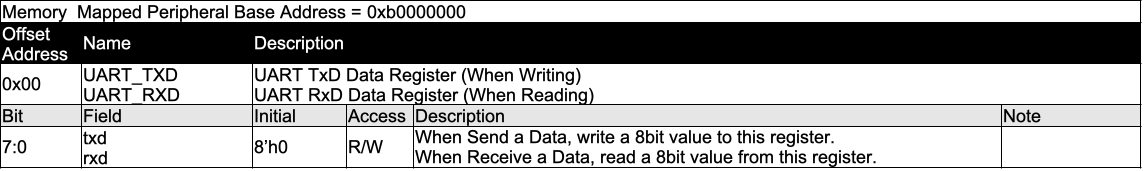
\includegraphics[width=1.0\columnwidth]{./Table/REG_UART_TXDRXD.png}
    \caption{UART\_TXD / UART\_RXD}
    \label{tb:REG_UART_TXDRXD}
\end{table}
%-------------------------------
%-------------------------------
\begin{table}[H]
    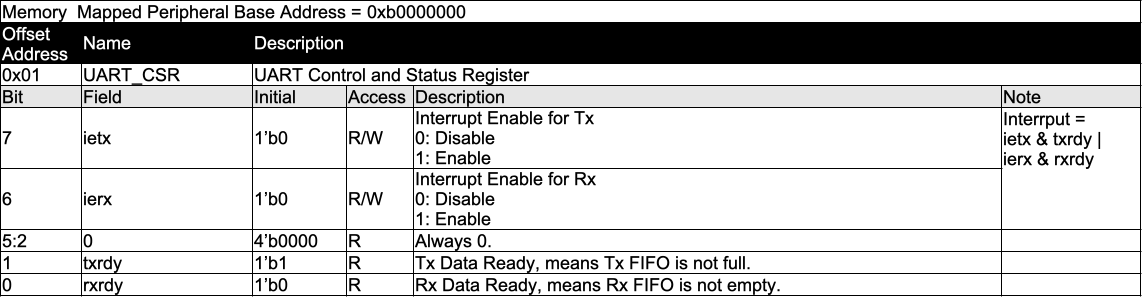
\includegraphics[width=1.0\columnwidth]{./Table/REG_UART_CSR.png}
    \caption{UART\_CSR}
    \label{tb:REG_UART_CSR}
\end{table}
%-------------------------------
%-------------------------------
\begin{table}[H]
    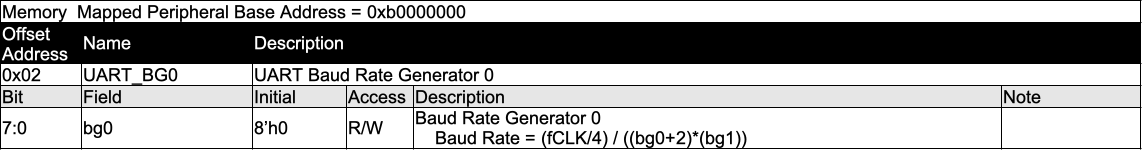
\includegraphics[width=1.0\columnwidth]{./Table/REG_UART_BG0.png}
    \caption{UART\_BG0}
    \label{tb:REG_UART_BG0}
\end{table}
%-------------------------------
%-------------------------------
\begin{table}[H]
    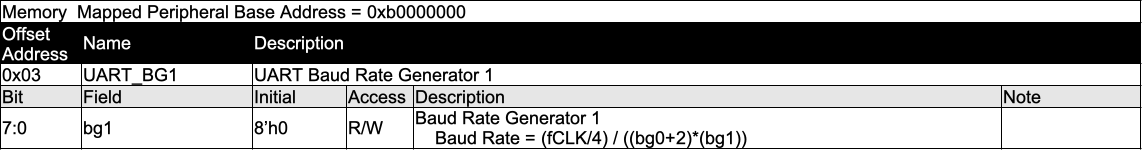
\includegraphics[width=1.0\columnwidth]{./Table/REG_UART_BG1.png}
    \caption{UART\_BG1}
    \label{tb:REG_UART_BG1}
\end{table}
%-------------------------------

